\documentclass[a4paper]{article}

\title{Sweave Example 1}

\author{Friedrich Leisch}

\usepackage{/Library/Frameworks/R.framework/Resources/share/texmf/Sweave}
\begin{document}

\maketitle

In this example we embed parts of the examples from the


\begin{Schunk}
\begin{Sinput}
> a = runif(1000)
> print(summary(a))
\end{Sinput}
\begin{Soutput}
     Min.   1st Qu.    Median      Mean   3rd Qu.      Max. 
2.984e-05 2.444e-01 5.236e-01 5.019e-01 7.499e-01 1.000e+00 
\end{Soutput}
\end{Schunk}

which shows that the location parameter of the Ozone

distribution varies significantly from month to month . Finally we

include a boxplot of the data :

\begin{center}
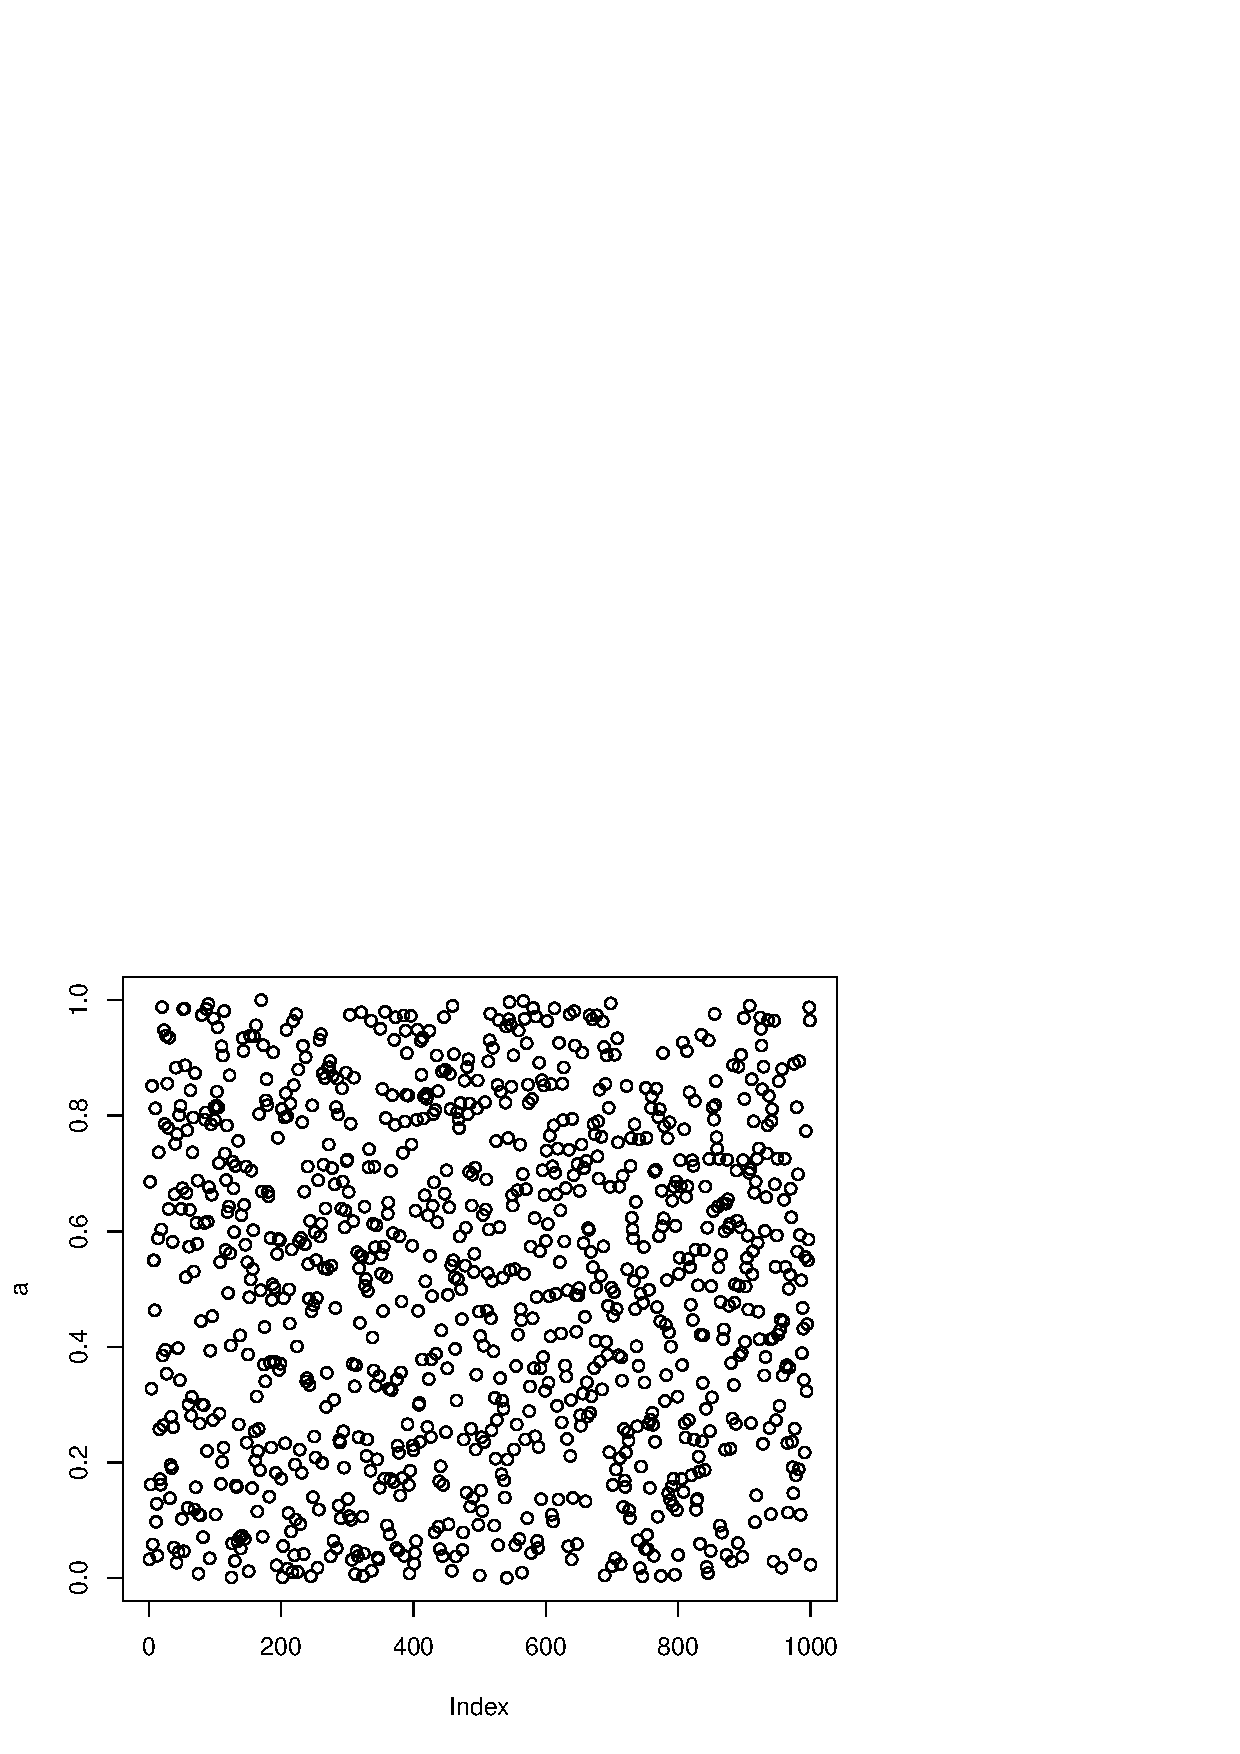
\includegraphics{example-002}

\end{center}

\end{document}
